\documentclass[tikz]{standalone}
\usepackage{tikz}
\usepackage{fourier}
\usepackage{physics}
\usetikzlibrary{shapes.geometric}
\usetikzlibrary{calc}

\begin{document}
\begin{tikzpicture}
    % Spherical harmonic plots
    \node[inner sep=0] at (0, 0) {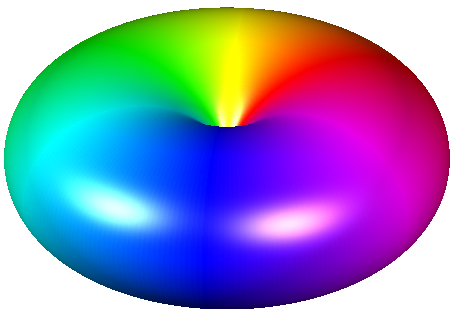
\includegraphics{gfx/FM-spherical.pdf}};
    \node[inner sep=0] at (7, 0) {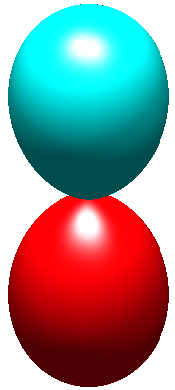
\includegraphics{gfx/polar-spherical.pdf}};
    \node[inner sep=0] at (15, 0) {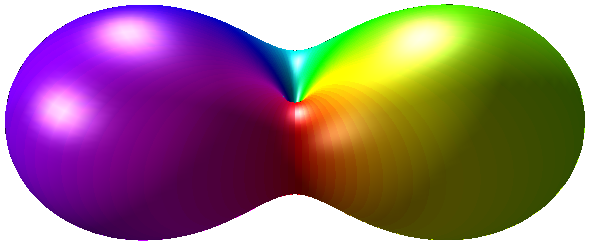
\includegraphics{gfx/AFM-spherical.pdf}};
    \node[inner sep=0] at (24, 0) {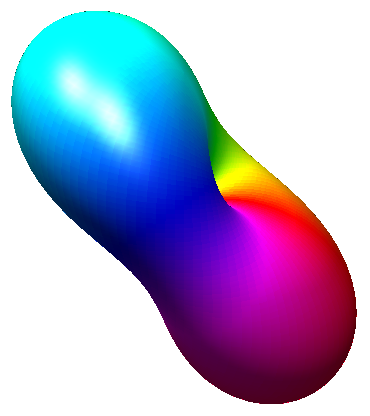
\includegraphics{gfx/BA-spherical.pdf}};

    % Colour bar
    \node[rotate=90] at (-5, 0) {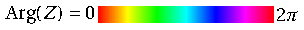
\includegraphics[scale=1.8]{gfx/compiled_hsv.pdf}};
    
    % Magnetisation & director lines
    \draw[->, dashed, line width=2] (0, 0.45) -- (0, 3.2);
    \draw[-, line width=2] (7, 3.2) -- (7, 4.2) node[above] {\Huge \(\hat{\vb{d}}\)};
    \draw[->, line width=2] (15, 0.3) -- (15, 2.2);
    \draw[->, line width=2] (24.5, 0.45) -- (25.5, 1.3);

    % Polar axis of symmetry and text
    \draw[->, line width=2] (7, -0.05) -- (8.5, -0.05) node[right] {\Huge \(C_2\)};
    

    % Subfigure labels
    \node at (0, -4) {\Huge (a)};
    \node at (7, -4) {\Huge (b)};
    \node at (15, -4) {\Huge (c)};
    \node at (24, -4) {\Huge (d)};

    % Axis orientation
    \draw[->, line width=2] (-3.5, -4) -- (-3.5, -3) node[above] {\LARGE \(z\)};
    \draw[->, line width=2] (-3.5, -4) -- (-2.5, -4) node[right] {\LARGE \(x\)};
    \draw[->, line width=2] (-3.5, -4) -- (-3, -3.5) node[right] {\LARGE \(y\)};
\end{tikzpicture}
\end{document}
